% GNUPLOT: LaTeX picture with Postscript
\begingroup
  \makeatletter
  \providecommand\color[2][]{%
    \GenericError{(gnuplot) \space\space\space\@spaces}{%
      Package color not loaded in conjunction with
      terminal option `colourtext'%
    }{See the gnuplot documentation for explanation.%
    }{Either use 'blacktext' in gnuplot or load the package
      color.sty in LaTeX.}%
    \renewcommand\color[2][]{}%
  }%
  \providecommand\includegraphics[2][]{%
    \GenericError{(gnuplot) \space\space\space\@spaces}{%
      Package graphicx or graphics not loaded%
    }{See the gnuplot documentation for explanation.%
    }{The gnuplot epslatex terminal needs graphicx.sty or graphics.sty.}%
    \renewcommand\includegraphics[2][]{}%
  }%
  \providecommand\rotatebox[2]{#2}%
  \@ifundefined{ifGPcolor}{%
    \newif\ifGPcolor
    \GPcolorfalse
  }{}%
  \@ifundefined{ifGPblacktext}{%
    \newif\ifGPblacktext
    \GPblacktexttrue
  }{}%
  % define a \g@addto@macro without @ in the name:
  \let\gplgaddtomacro\g@addto@macro
  % define empty templates for all commands taking text:
  \gdef\gplbacktext{}%
  \gdef\gplfronttext{}%
  \makeatother
  \ifGPblacktext
    % no textcolor at all
    \def\colorrgb#1{}%
    \def\colorgray#1{}%
  \else
    % gray or color?
    \ifGPcolor
      \def\colorrgb#1{\color[rgb]{#1}}%
      \def\colorgray#1{\color[gray]{#1}}%
      \expandafter\def\csname LTw\endcsname{\color{white}}%
      \expandafter\def\csname LTb\endcsname{\color{black}}%
      \expandafter\def\csname LTa\endcsname{\color{black}}%
      \expandafter\def\csname LT0\endcsname{\color[rgb]{1,0,0}}%
      \expandafter\def\csname LT1\endcsname{\color[rgb]{0,1,0}}%
      \expandafter\def\csname LT2\endcsname{\color[rgb]{0,0,1}}%
      \expandafter\def\csname LT3\endcsname{\color[rgb]{1,0,1}}%
      \expandafter\def\csname LT4\endcsname{\color[rgb]{0,1,1}}%
      \expandafter\def\csname LT5\endcsname{\color[rgb]{1,1,0}}%
      \expandafter\def\csname LT6\endcsname{\color[rgb]{0,0,0}}%
      \expandafter\def\csname LT7\endcsname{\color[rgb]{1,0.3,0}}%
      \expandafter\def\csname LT8\endcsname{\color[rgb]{0.5,0.5,0.5}}%
    \else
      % gray
      \def\colorrgb#1{\color{black}}%
      \def\colorgray#1{\color[gray]{#1}}%
      \expandafter\def\csname LTw\endcsname{\color{white}}%
      \expandafter\def\csname LTb\endcsname{\color{black}}%
      \expandafter\def\csname LTa\endcsname{\color{black}}%
      \expandafter\def\csname LT0\endcsname{\color{black}}%
      \expandafter\def\csname LT1\endcsname{\color{black}}%
      \expandafter\def\csname LT2\endcsname{\color{black}}%
      \expandafter\def\csname LT3\endcsname{\color{black}}%
      \expandafter\def\csname LT4\endcsname{\color{black}}%
      \expandafter\def\csname LT5\endcsname{\color{black}}%
      \expandafter\def\csname LT6\endcsname{\color{black}}%
      \expandafter\def\csname LT7\endcsname{\color{black}}%
      \expandafter\def\csname LT8\endcsname{\color{black}}%
    \fi
  \fi
  \setlength{\unitlength}{0.0500bp}%
  \begin{picture}(4000.00,3000.00)%
    \gplgaddtomacro\gplbacktext{%
      \colorrgb{0.00,0.00,0.00}%
      \put(388,1822){\makebox(0,0)[r]{\strut{}\small $0$}}%
      \colorrgb{0.00,0.00,0.00}%
      \put(388,1981){\makebox(0,0)[r]{\strut{}\small $200$}}%
      \colorrgb{0.00,0.00,0.00}%
      \put(388,2139){\makebox(0,0)[r]{\strut{}\small $400$}}%
      \colorrgb{0.00,0.00,0.00}%
      \put(388,2298){\makebox(0,0)[r]{\strut{}\small $600$}}%
      \colorrgb{0.00,0.00,0.00}%
      \put(388,2457){\makebox(0,0)[r]{\strut{}\small $800$}}%
      \colorrgb{0.00,0.00,0.00}%
      \put(388,2615){\makebox(0,0)[r]{\strut{}\small $1000$}}%
      \colorrgb{0.00,0.00,0.00}%
      \put(388,2774){\makebox(0,0)[r]{\strut{}\small $1200$}}%
      \colorrgb{0.00,0.00,0.00}%
      \put(778,1602){\makebox(0,0){\strut{}}}%
      \colorrgb{0.00,0.00,0.00}%
      \put(1037,1602){\makebox(0,0){\strut{}}}%
      \colorrgb{0.00,0.00,0.00}%
      \put(1295,1602){\makebox(0,0){\strut{}}}%
      \colorrgb{0.00,0.00,0.00}%
      \put(1553,1602){\makebox(0,0){\strut{}}}%
      \colorrgb{0.00,0.00,0.00}%
      \put(1811,1602){\makebox(0,0){\strut{}}}%
      \colorrgb{0.00,0.00,0.00}%
      \put(2070,1602){\makebox(0,0){\strut{}}}%
      \colorrgb{0.00,0.00,0.00}%
      \put(2328,1602){\makebox(0,0){\strut{}}}%
      \colorrgb{0.00,0.00,0.00}%
      \put(2586,1602){\makebox(0,0){\strut{}}}%
      \colorrgb{0.00,0.00,0.00}%
      \put(2844,1602){\makebox(0,0){\strut{}}}%
      \colorrgb{0.00,0.00,0.00}%
      \put(3103,1602){\makebox(0,0){\strut{}}}%
      \colorrgb{0.00,0.00,0.00}%
      \put(3361,1602){\makebox(0,0){\strut{}}}%
      \colorrgb{0.00,0.00,0.00}%
      \put(-646,2298){\rotatebox{90}{\makebox(0,0){\strut{}PL-ICP}}}%
      \colorrgb{0.00,0.00,0.00}%
      \put(2069,3104){\makebox(0,0){\strut{}Mean execution time [ms]}}%
    }%
    \gplgaddtomacro\gplfronttext{%
    }%
    \gplgaddtomacro\gplbacktext{%
      \colorrgb{0.00,0.00,0.00}%
      \put(388,330){\makebox(0,0)[r]{\strut{}\small $0$}}%
      \colorrgb{0.00,0.00,0.00}%
      \put(388,489){\makebox(0,0)[r]{\strut{}\small $200$}}%
      \colorrgb{0.00,0.00,0.00}%
      \put(388,647){\makebox(0,0)[r]{\strut{}\small $400$}}%
      \colorrgb{0.00,0.00,0.00}%
      \put(388,806){\makebox(0,0)[r]{\strut{}\small $600$}}%
      \colorrgb{0.00,0.00,0.00}%
      \put(388,965){\makebox(0,0)[r]{\strut{}\small $800$}}%
      \colorrgb{0.00,0.00,0.00}%
      \put(388,1123){\makebox(0,0)[r]{\strut{}\small $1000$}}%
      \colorrgb{0.00,0.00,0.00}%
      \put(388,1282){\makebox(0,0)[r]{\strut{}\small $1200$}}%
      \colorrgb{0.00,0.00,0.00}%
      \put(778,110){\makebox(0,0){\strut{}\small $\bm{p}_a^A$}}%
      \colorrgb{0.00,0.00,0.00}%
      \put(1037,110){\makebox(0,0){\strut{}\small $\bm{p}_b^A$}}%
      \colorrgb{0.00,0.00,0.00}%
      \put(1295,110){\makebox(0,0){\strut{}\small $\bm{p}_c^A$}}%
      \colorrgb{0.00,0.00,0.00}%
      \put(1553,110){\makebox(0,0){\strut{}\small $\bm{p}_d^A$}}%
      \colorrgb{0.00,0.00,0.00}%
      \put(1811,110){\makebox(0,0){\strut{}\small $\bm{p}_e^A$}}%
      \colorrgb{0.00,0.00,0.00}%
      \put(2070,110){\makebox(0,0){\strut{}\small $\bm{p}_f^A$}}%
      \colorrgb{0.00,0.00,0.00}%
      \put(2328,110){\makebox(0,0){\strut{}\small $\bm{p}_g^A$}}%
      \colorrgb{0.00,0.00,0.00}%
      \put(2586,110){\makebox(0,0){\strut{}\small $\bm{p}_h^A$}}%
      \colorrgb{0.00,0.00,0.00}%
      \put(2844,110){\makebox(0,0){\strut{}\small $\bm{p}_i^A$}}%
      \colorrgb{0.00,0.00,0.00}%
      \put(3103,110){\makebox(0,0){\strut{}\small $\bm{p}_j^A$}}%
      \colorrgb{0.00,0.00,0.00}%
      \put(3361,110){\makebox(0,0){\strut{}\small $\bm{p}_k^A$}}%
      \colorrgb{0.00,0.00,0.00}%
      \put(-646,806){\rotatebox{90}{\makebox(0,0){\strut{}PGL-FMIC}}}%
      \colorrgb{0.00,0.00,0.00}%
      \put(2069,-220){\makebox(0,0){\strut{}Identifier of tested pose in real environment CSAL}}%
    }%
    \gplgaddtomacro\gplfronttext{%
    }%
    \gplbacktext
    \put(0,0){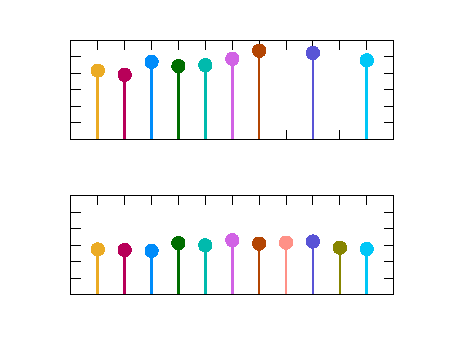
\includegraphics{/home/li9i/catkin_ws/src/relief_fmt_global_localisation/experiments_logs/evaluation_scripts_phd/figures/csal_execution_times}}%
    \gplfronttext
  \end{picture}%
\endgroup
